\subsection{Design of the Data Management}\label{subsec:backend_datamanagement}

Gathering and structuring the data in this project is quite a challenge. The stores and retailers do not publish the prices of all their products, they only issue a catalog with items on sale. These items on sale, or offers, are published in a new catalog each week. The figure \ref{fig:backend_dataflow} shows the complete design of the dataflow for our solution. It illustrates the complexity of gathering information from different sources and presenting them to the user. Recipes have to be gathered from a free website or from the users using the application. But a base source of recipes is also needed, to enable people to actually use the application in the first place. These database entries with actual recipes needs to come from somewhere. \textit{Opskrifter.dk} is a huge online database with around 3.000 different recipes, and these are the recipes we intend to use and work with in our application. This part may seem like a rather trivial task, however adjusting recipes for spelling errors and matching them with the proper ingredients can be problem. This error checking and matching requires some difficult string analysis. It will be possible for us as the developers to control and maintain the data, but it does require a lot of the work, and most of it have to be done manually, because it is extremely challenging to catch all of the problems with the recipes.

In this project we need a strong foundation for the ingredient data. We want to match both recipes and offers to specific ingredients. This is what will allow the computations of costs, buying certain ingredients for a recipe, including ingredients on sale. Ingredient data is more complicated because no complete list exists. For the project, a data-sheet from Statistics Denmark  was bought, which can be seen in Appendix \ref{appendix:averageprices}). This contains average prices of groceries, across danish stores and retailers. Groceries can be ingredients or food items used to cook. We want to use these as a base for all calculations we do. All of this data works as a functioning base, but does however not portray a completely true image of each store and retailer. It will resolve in some values as to what you save and actual price, that wont be 100\% correct. As a result, our application may only be seen as a guidance and estimate of prices and savings, not guaranteeing exact prices. The offers for the different groceries are gathered through \textit{eTilbudsavis}. This online service gathers all offers offered by a selection of retailers in Denmark, and it does so by traversing the catalogs and extracting all the data. They offer all their data through a web based application programming interface (API), and the idea is that our backend downloads the relevant data from their database once a day, and perform the necessary operations for it to match our database. 

\begin{figure}
\centering
\includegraphics[width=0.95\textwidth]{Pictures/dataflow}
\caption{A model of the dataflow through the entire system}
\label{fig:backend_dataflow}
\end{figure}

\paragraph{Design of the Database}
\label{para:dbdesign}

Data is a big part of this project. Data is content, data is what makes the users want to start, and continue using the application. Obviously the data should be handled in a uniform and structured way, which is the reason why we designed and implemented a database. A big part of the application is dependent upon the database being frequently and correctly updated. Furthermore the database has to be designed in a way that makes calculations fast to compute and access, as we do not want the user to wait for too long in order to get something shown on the application. We will have big amounts of data, with a daily update requirement and social media storage requirements for talking about recipes.

When we design our database, we want to achieve a goal that is to keep the database as simple as possible. We do not want to have unnecessary entities or large amount of attributes in a single table. With our desire to provide query-results quickly, we also want to split data into separate tables, and by that allow search for specific data in outlined tables. 

We found the need for five entities, each rather self-explanatory but they will be briefly described:

\paragraph{Account} Used to hold an account created by a user of the application. It is needed to store the actions and changes made by a user while using the application. 

\paragraph{Recipe} Used to store the main information about a recipe, e.g. how to cook it. This alone does not tell the user what ingredients to use.

\paragraph{Comment} Used to store a users opinion in context of a recipe.

\paragraph{Ingredient} Used to store the entire list of ingredients known by the application. This does not tell the user which ingredient is part of what recipe.

\paragraph{Retailer} Used to store the different types of retailers offering groceries, and all of their individual stores and locations.
\newline

\begin{figure}
\centering
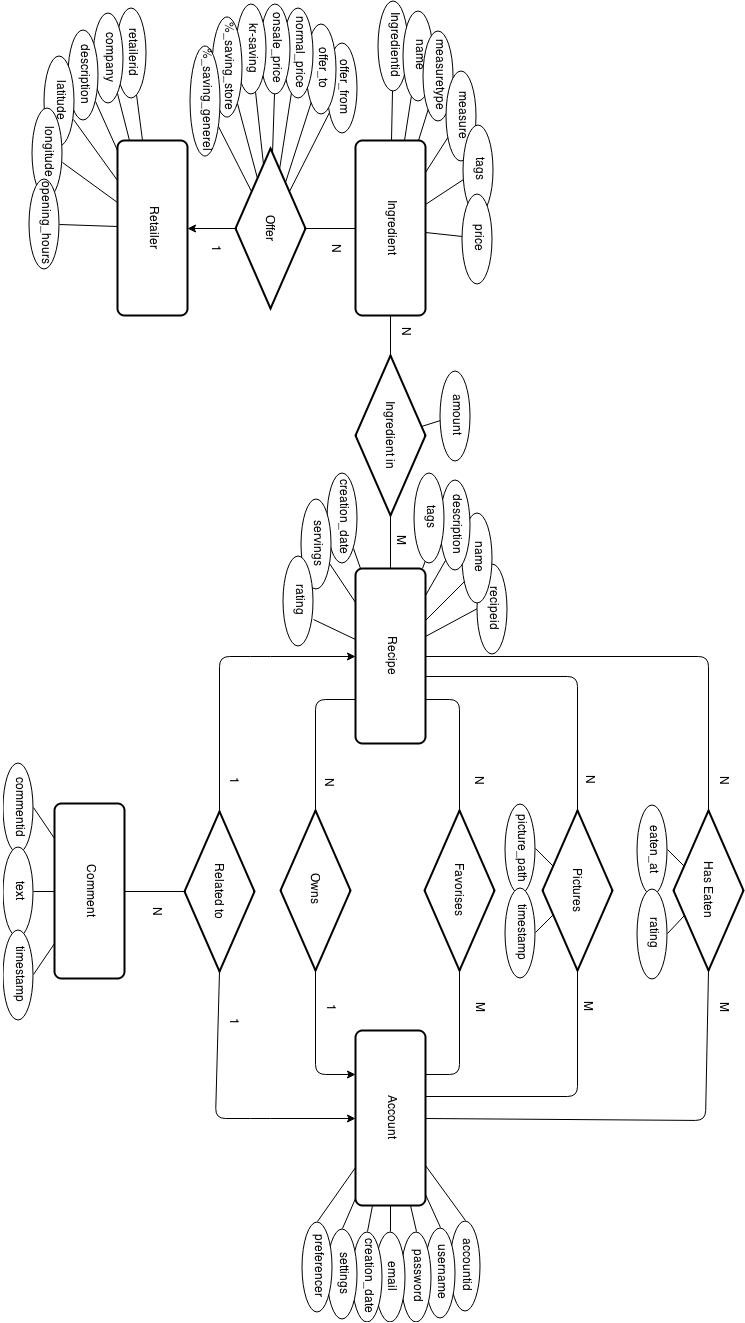
\includegraphics[width=0.95\textwidth]{Pictures/ERdiagram}
\caption{The final ER diagram of the database}
\label{fig:ER-diagram}
\end{figure}

Entities do not provide much use without connecting them and giving their interactions a sense of purpose. Therefore we define relationships among entities to allow different interactions and give the user a way to store the functionality provided in the application. An example of this functionality could be the possibility to favor a recipe, and hereby keeping a list of favored recipes. Clicking a button to save a favorite does not make sense unless the action is stored in the database. Therefore we designed a relationship between \textit{Account} and \textit{Recipe} called \textit{Favorises} that stores this data.

We have a total of 7 relationships in the ER diagram. If we continued without optimizing, we would have had a database with 12 tables. But since we mapped the ER diagram to relations, we eliminated the need for two tables, and ended up with a relational schema looking like this:

\begin{itemize}
\item \textbf{Accounts} (\underline{accountid}, email, password, alias, creatingdate, settings, preferences)
%
\item \textbf{Comments} ( \underline{commentid, recipeid → Recipe}, accountid → Account, creationdate, text)

\item \textbf{Favorises} (\underline{accountid → Account, recipeid → Recipe})

\item \textbf{HasEaten} (\underline{accountid → Account, recipeid → Recipe}, eatenat, rating)

\item \textbf{Ingredients} (\underline{ingredientid}, name, measurementtype, measure, price, organic, fat, fresh)

\item \textbf{IngredientIn} (\underline{ingrendientid → Ingredient, recipeid → Recipe}, amount)

\item \textbf{Offers} (\underline{retailerid → Retailer, ingredientid → Ingredient}, offerfrom, offerto, normalprice, onsaleprice, krsaving, percentagesavingretailer, percentagesavinggeneral)

\item \textbf{Pictures} (\underline{accountid → Account, recipeid → Recipe}, picturepath, creationdate)

\item \textbf{Recipes} (\underline{recipeid}, accountid → Account, name, description, creationdate, numberofservings, rating)

\item \textbf{Retailers} (\underline{retailerid, latitude, longitude}, companyname, description, openinghours)
\end{itemize}

During the process of working with the database, we discovered the need to store tags for recipes and ingredients. Storing tags as a large string on a single recipe or ingredient is highly inefficient because one of the worst performance sinks in database queries is string comparison. Therefore we created two extra tables to store tags, and their relational schema look as below:

\begin{itemize}
\item \textbf{Recipetags} (\underline{recipeid → Recipe, tag})

\item \textbf{Ingredienttags} (\underline{ingredientid → Ingredient, tag}) 
\end{itemize}

These tables are not shown in the ER diagram, but are attached as weak-entity relationships to both recipe and ingredient. This makes querying easy. You can query for a recipe and the attached tags, or search for a specific tag and return matching recipes as the result.

A lot of these relations speak for themselves, and the entire amount of relationships between account and recipe is rather intuitive. We have chosen not to gather all the data in a single relationship as we want perform quick queries on the database rather than save memory. This is one of the advantages of having a backend with a large amount of memory available, it is possible to focus primarily on performance. Alternatively, we would have to make heavy computations on a mobile device with limited resources which is undesirable.